\chapter{Introducing ANTLR}
If your task is to implement a parser, it is best to use one of the tools that is available for this purpose.
The wikipedia page 
\href{https://en.wikipedia.org/wiki/Comparison_of_parser_generators}{Comparison of parser generators}
shows the large number of \blue{parser generators} that are available.  
A \blue{parser generator} \index{parser generator}\index{parser generator} is a program that takes a grammar as
its input and generates a parser that can parse according to this grammar.
In my opinion, the parser generator that is both most mature\footnote{
  The first version of \textsc{Antlr} became available in 1992 and \textsc{Antlr} 4.0 was released in 2012.
} and most powerful is
\textsc{Antlr} \index{\textsc{Antlr}} \cite{parr:2012,parr:2014}.  The name is short for 
\emph{\underline{an}other \underline{t}ool for \underline{l}anguage \underline{r}ecognition}\footnote{
  The name \textsc{Antlr} can also be interpreted as an acronym for \underline{ant}i \underline{LR},
  where ``LR'' is short for \emph{LR} parser.  LR parsers are a kind of \emph{bottom-up parsers}.  We will discuss these
  parsers later in chapter \ref{chapter:bottom-up}.
}.
\textsc{Antlr} can be downloaded at 
\\[0.2cm]
\hspace*{1.3cm}
\href{http://www.antlr.org}{\texttt{http://www.antlr.org}}.
\\[0.2cm]
In this lecture we will use \textsc{Antlr} version 4.8, which was released in January 2020.  The tool \textsc{Antlr} is written in \textsl{Java}
and therefore its main target language is \textsl{Java}.  However, \textsc{Antlr} can also be used to generate
parsers for the programming languages \texttt{C++}, \texttt{C\#}, \textsl{Python}, \textsl{JavaScript},
\textsl{Go}, and \textsl{Swift}. 
We will introduce \textsc{Antlr} via some examples that demonstrate the most important features of this tool.
For a discussion of all the features offered by \textsc{Antlr} I recommend the book 
``The Definitive \textsc{Antlr} Reference'' by Terrence Parr \cite{parr:2012}.  However, this book only covers
the generation of \textsl{Java} parsers. 

\section{A Parser for Arithmetic Expressions}
We start with a parser for arithmetic expressions.  The structure of arithmetic expressions can be described by
the grammar that is shown in Figure \ref{fig:Expr} on page \pageref{fig:Expr}.
If we use \textsc{Antlr} we can implement this grammar as shown in Figure \ref{fig:Expr.g4}.  
We discuss the implementation line by line.

\begin{figure}[!ht]
\centering
\begin{minted}[ frame         = lines, 
                framesep      = 0.3cm, 
                numbers       = left,
                numbersep     = -0.2cm,
                bgcolor       = sepia,
                xleftmargin   = 0.8cm,
                xrightmargin  = 0.8cm,
              ]{antlr}
    grammar Expr;
    
    start   : expr
            ;
    
    expr    : expr '+' product 
            | expr '-' product
            | product        
            ;
    
    product : product '*' factor 
            | product '/' factor 
            | factor
            ;
    
    factor  : '(' expr ')'
            | NUMBER
            ;
    
    NUMBER  : '0'|[1-9][0-9]*;
    WS      : [ \t\n\r] -> skip;
\end{minted}
\vspace*{-0.3cm}
\caption{\textsc{Antlr} grammar for arithmetical expressions.}
\label{fig:Expr.g4}
\end{figure}


\begin{enumerate}
\item In line 1 the keyword \texttt{grammar} specifies the name of the grammar.
      In this case the grammar is called \texttt{Expr}.  This grammar has to be stored in a file with the name 
      ``\texttt{Expr.g4}''.  The rule is that the file name has to be the same name as the name of the grammar
      and the file extension has to be ``\texttt{.g4}''.  
\item Line 3 gives the grammar rule for the non-terminal \textsl{start}.  In the last chapter we would have used the
      notation \\[0.2cm]
      \hspace*{1.3cm}
      $\textsl{start} \rightarrow \textsl{expr}$
      \\[0.2cm]
      to specify this rule.  With \textsc{Antlr} the left and right part of a grammar rule are separated by a colon.
      \textsc{Antlr} terminates every grammar rule with the character ``\texttt{;}''.
\item Line 6--9 give the grammar rules for the non-terminal \textsl{expr}.  Note that we have to enclose the 
      terminals ``\texttt{+}'' and ``\texttt{-}'' in single quotes.  The different alternatives for the non-terminal
      \texttt{expr} are separated by the character ``\texttt{|}''.
\item Similarly, the lines 11--14 and 16--18 show the grammar rules for the non-terminals \textsl{product} and
      \textsl{factor}.   
\item With \textsc{Antlr} the grammar and the specification of the tokens can be given in the same file.
      In order to be able to distinguish terminals and non-terminals, terminals have to begin with an upper case 
      letter,\footnote
      {It is a convention that the names of non-terminals consist of only upper case letters, but this is not required.}
      while non-terminals start with a lower case letter.   Therefore, ``\texttt{NUMBER}'' is the name
      of a terminal.
\item In line 20 the lexical specification of the non-terminal \texttt{NUMBER} is given
      by a regular expression.  The regular expression
      \\[0.2cm]
      \hspace*{1.3cm}
      \texttt{'0'|[1-9][0-9]*;}
      \\[0.2cm]
      describes a sequence of digits.  This sequence can only start with the digit
      ``\texttt{0}'' when ``\texttt{0}'' not followed by any other digit.

      Notice that we have to enclose the first occurrence of ``\texttt{0}'' in single quotes.
      On the other hand, we must not put the digits occurring in the square brackets ``\texttt{[}'' 
      and ``\texttt{]}'' in quotes, since these occur inside a \blue{range} and characters inside a range
      must never be quoted.
\item Line 21 defines the terminal \texttt{WS}, where the name \texttt{WS} is short for \emph{white space}. This terminal
      specifies a single character that is either a blank, a tabulator, a line break, or a carriage return.
      The lexical specification of the terminal \texttt{WS} is followed by the operator ``\texttt{->}'' 
      which in turn is followed by a \blue{semantic action}.
      The semantic action ``\texttt{skip}'', which is executed once a white space character has been recognized, 
      simply discards the white space character.  Therefore, the net effect of line 21 is to discard all white
      space characters. 

      In most programming languages\footnote{
        Unfortunately, \textsl{Python} is an exception to this rule.  Therefore, parsing
        \textsl{Python} is considerably harder than parsing languages like \texttt{C} or \textsl{Java}.
      }, white space has no purpose other than that of separating  tokens.  
      Therefore, most \textsc{Antlr} parsers will have a scanner rule that is similar to
      the rule shown in line 21. 
\end{enumerate}
To conclude, the lines 3--18 specify the grammar, while the lines 20--21 specify the 
lexical structure.  If the grammar that is shown in Figure \ref{fig:Expr.g4} is stored in the file
\href{https://github.com/karlstroetmann/Formal-Languages/blob/master/ANTLR4-Python/PureExprParser/Expr.g4}{\texttt{Expr.g4}} 
we can generate a parser by using the following command:
\\[0.2cm]
\hspace*{1.3cm}
\texttt{java -jar /usr/local/lib/antlr-4.8-complete.jar -Dlanguage=Python3 Expr.g4}
\\[0.2cm]
Of course, this only works if the file \texttt{antlr-4.8-complete.jar} is stored in the directory
\texttt{/usr/local/lib/}.  Among others, \texttt{Antlr} will then generate the following files:
\begin{enumerate}
\item \texttt{ExprParser.py}

      This file contains the parser.
\item \texttt{ExprLexer.py}

      This is the scanner.
\item \textsc{Antlr} generates some more files.  However, these are not relevant for us.
\end{enumerate}

In order to run the parser we need a driver program.  Figure \ref{fig:PureParser.ipynb} shows such a program.

\begin{figure}[!ht]
\centering
\begin{minted}[ frame         = lines, 
                framesep      = 0.3cm, 
                bgcolor       = sepia,
                numbers       = left,
                numbersep     = -0.2cm,
                xleftmargin   = 0.8cm,
                xrightmargin  = 0.8cm,
              ]{python}
    from ExprLexer  import ExprLexer
    from ExprParser import ExprParser
    
    import antlr4
    
    def parse_string(string): 
        inputStream = antlr4.InputStream(string)
        lexer       = ExprLexer(inputStream)
        tokenStream = antlr4.CommonTokenStream(lexer)
        parser      = ExprParser(tokenStream)
        parser.start()
\end{minted}
\vspace*{-0.3cm}
\caption{Driver program for the parser generated by \textsc{Antlr}.}
\label{fig:PureParser.ipynb}
\end{figure}

\begin{enumerate}
\item In Line 1 and 2 we import the scanner and the parser that has been generated by \textsc{Antlr}.
\item Line 7 transforms the input from a string into an object of class \texttt{InputStream}.
      This object is then used to create the scanner \texttt{lexer}.
\item Using this scanner we create an object of class \texttt{CommonTokenStream}.
      This object is then fed into the parser in line 10.
\item The parser is called in line 11.  In order to call the parser we have to invoke the method 
      \texttt{start}.  Here \texttt{start} is the name of the non-terminal that is to be recognized
\end{enumerate}
If we want to test our parser we use the command:
\\[0.2cm]
\hspace*{1.3cm}
\texttt{parse\_string(\symbol{34}1 + 2 * 3 - 4\symbol{34})}
\\[0.2cm]
This will run without errors, showing that the input string adheres to the specification of the grammar.
If we want to see the parse tree instead, we have to use the \texttt{TestRig} provided by \textsc{Antlr}.
In order to use the \texttt{TestRig}, we first have to create a \textsl{Java}-based parser using the command
\\[0.2cm]
\hspace*{1.3cm}
\texttt{java -jar /usr/local/lib/antlr-4.8-complete.jar -Dlanguage=Java Expr.g4}
\\[0.2cm]
The generated \textsl{Java} files have to be compiled with the following command:
\\[0.2cm]
\hspace*{1.3cm}
\texttt{javac -cp .:/usr/local/lib/antlr-4.8-complete.jar *.java}
\\[0.2cm]
After that we can generate a parse tree using the command
\\[0.2cm]
\hspace*{0.3cm}
\texttt{java -cp .:/usr/local/lib/antlr-4.8-complete.jar org.antlr.v4.gui.TestRig Expr start -gui}
\\[0.2cm]
This command will open a tree viewer that shows the parse tree of any input we have typed in response to this command.
For the input string ``\texttt{1 + 2 * 3 - 4}''  this tree looks as shown in Figure \ref{fig:parse-tree.pdf}.

\begin{figure}[!ht]
  \centering
      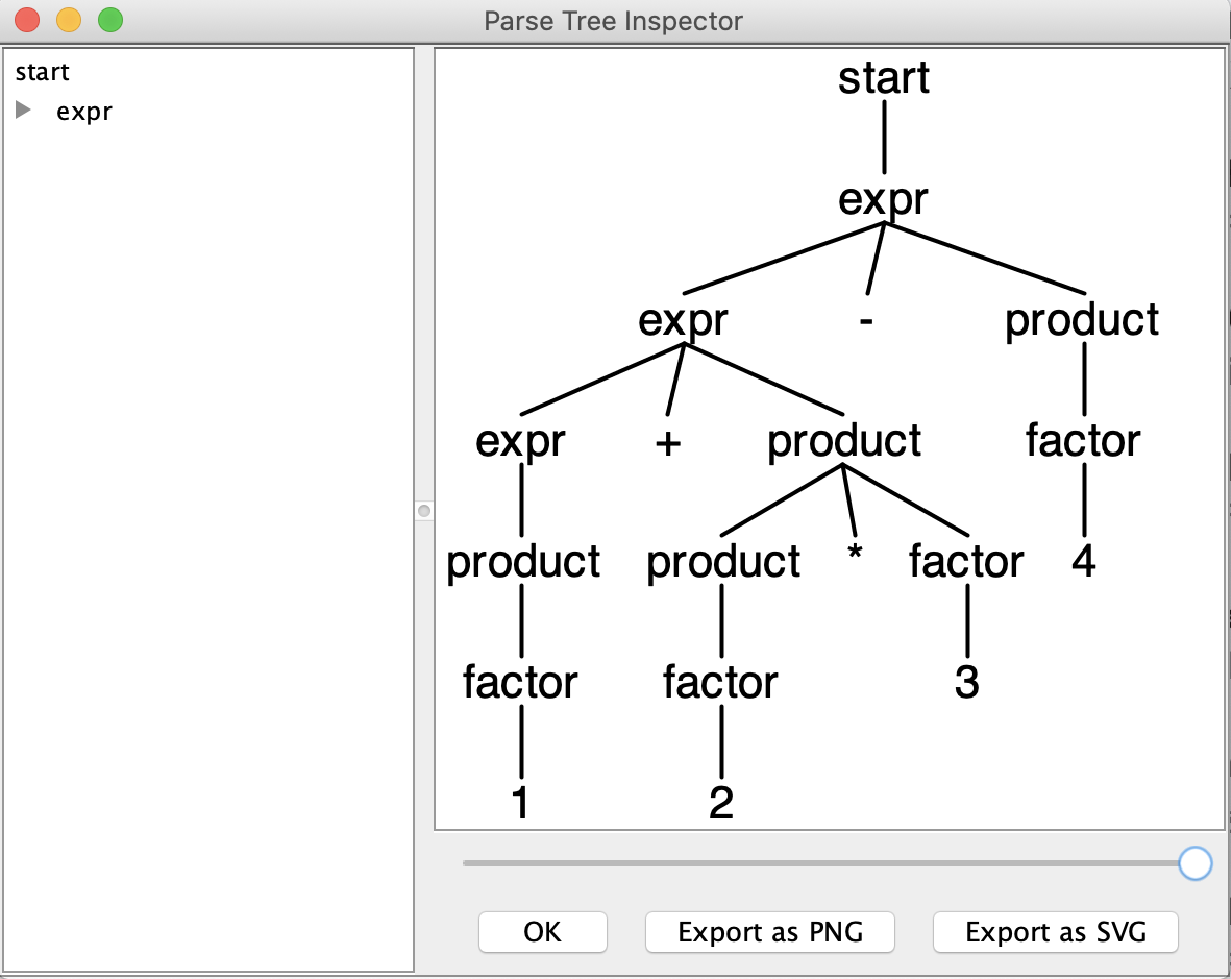
\epsfig{file=Abbildungen/parse-tree.pdf, scale=0.7}
   \caption{Parse tree for the string ``\texttt{1 + 2 * 3 - 4}''.}
  \label{fig:parse-tree.pdf}
\end{figure}



\section{Evaluation of Arithmetical Expressions}
The last example isn't very exciting as the arithmetical expressions that the parser reads are not
evaluated.  In this section we show how arithmetical expressions can be evaluated using \textsc{Antlr}
generated parsers.  We proceed in two steps:
\begin{enumerate}
\item Firstly, we present a grammar for a small symbolic calculator.
\item Secondly, we show how this grammar can be extended with actions so that the expressions can be evaluated.
\end{enumerate}
Figure \ref{fig:Program.g4} presents the grammar.  In comparison with grammar for arithmetical expressions that
was shown in Figure \ref{fig:Expr.g4} there are the following changes:

\begin{figure}[!ht]
\centering
\begin{minted}[ frame         = lines, 
                framesep      = 0.3cm, 
                bgcolor       = sepia,
                numbers       = left,
                numbersep     = -0.2cm,
                xleftmargin   = 0.8cm,
                xrightmargin  = 0.8cm,
              ]{antlr}
    grammar Program;
    
    start: statement+ ; 
    
    statement
        : IDENTIFIER ':=' expr ';' 
        | expr ';'                 
        ;
    
    expr: expr '+' product 
        | expr '-' product 
        | product
        ;
    
    product 
        : product '*' factor 
        | product '/' factor 
        | factor
        ;
    
    factor
        : 'sqrt' '(' expr ')'
        | '(' expr ')'        
        | FLOAT               
        | IDENTIFIER          

        ;
    
    IDENTIFIER: [a-zA-Z][a-zA-Z0-9_]*;
    FLOAT     : '0'([.][0-9]+)?
              | [1-9][0-9]*([.][0-9]+)?
              ;
    WS        : [ \t\n\r] -> skip; 
\end{minted}
\vspace*{-0.3cm}
\caption{A grammar for a symbolic calculator.}
\label{fig:Program.g4}
\end{figure}


\begin{enumerate}
\item Das Start-Symbol \texttt{start} now recognizes a list of \blue{statements}.
      Note that \textsc{Antlr} provides the postfix operator ``\texttt{+}'' to
      specify non-empty sequences.  The postfix operators ``\texttt{*}'' and ``\texttt{?}'' are also 
      supported.  They have the same semantics as in regular expressions.
\item A \texttt{statement} is either an assignment or an expression.
\item The rules for expressions and products are the same as previously.
\item The rule for the non-terminal \texttt{factor} has changed.
      \begin{enumerate}[(a)]
      \item We can still put expressions in parenthesis.
      \item Instead of integers the grammar now supports floating point numbers.
            These are recognized by the terminal \texttt{FLOAT}.
      \item Expressions can now contain variables.  These are recognized by the terminal
            \texttt{IDENTIFIER}.
      \item Furthermore, expressions are allowed to contain calls of the function \texttt{sqrt},
            which is supposed to compute the square root of a given number.
      \end{enumerate}
\item The terminal \texttt{IDENTIFIER} recognizes variable names.  A variable name starts with 
      a letter from the Latin alphabet, i.e. a character from the range \texttt{[a-z]}.  This letter can be either
      upper or lower case.  The remaining characters of a variable name can be either letters from the Latin
      alphabet, digits, or the underscore.
\item The terminal \texttt{FLOAT} recognizes floating point numbers, i.e. numbers that have an optional
      fractional part like $1.23$.  Note that the dot ``\texttt{.}'' has to be enclosed in square
      brackets because otherwise it would match any character that is different from a newline.  
\end{enumerate}
A parser for this grammar is able to parse strings like the following:
\begin{verbatim}
    x := 2.3 * 3.4; y := sqrt(2 * x); z := x * x + y * y; sqrt(z);
\end{verbatim}
Our next task is to develop an interpreter for the language specified by the grammar shown 
in Figure \ref{fig:Program.g4}.  Figure \ref{fig:Calculator.g4} shows how an interpreter can be realized using
\textsc{Antlr}. 


\begin{figure}[!ht]
\centering
\begin{minted}[ frame         = lines, 
                framesep      = 0.3cm, 
                numbers       = left,
                numbersep     = -0.2cm,
                bgcolor       = sepia,
                xleftmargin   = 0.3cm,
                xrightmargin  = 0.3cm,
              ]{antlr}
    grammar Calculator;
    
    @header {
    import math
    }
    
    start: statement+ ; 
    
    statement
        : IDENTIFIER ':=' expr ';' {self.Values[$IDENTIFIER.text] = $expr.result}
        | expr ';'                 {print($expr.result)                         }
        ;
    
    expr returns[result]
        : e=expr '+' p=product {$result = $e.result + $p.result}
        | e=expr '-' p=product {$result = $e.result - $p.result}
        | p=product            {$result = $p.result            }
        ;
    
    product returns[result]
        : p=product '*' f=factor {$result = $p.result * $f.result}
        | p=product '/' f=factor {$result = $p.result / $f.result}
        | f=factor               {$result = $f.result            }
        ;
    
    factor returns[result]
        : '(' expr ')'        {$result = $expr.result                 }
        | FLOAT               {$result = float($FLOAT.text)           }
        | IDENTIFIER          {$result = self.Values[$IDENTIFIER.text]}
        | 'sqrt' '(' expr ')' {$result = math.sqrt($expr.result)      }
        ;
    
    IDENTIFIER: [a-zA-Z][a-zA-Z0-9_]*;
    FLOAT     : '0'([.][0-9]+)?
              | [1-9][0-9]*([.][0-9]+)?;
    WS        : [ \t\n\r] -> skip; 
\end{minted}
%\$
\vspace*{-0.3cm}
\caption{An interpreter for evaluating arithmetical expressions.}
\label{fig:Calculator.g4}
\end{figure}

\begin{enumerate}
\item As we have to use the function \texttt{sqrt} that is located in the module \texttt{math}
      we need to import this module into our parser.
      This is achieved by the header declaration shown in line 3--5.  The header declaration
      is started with the keyword \texttt{\@header} that is followed by an opening brace.
      It ends at the matching closing brace.
      \textsc{Antlr} puts all the code that is between the braces at the beginning of the generated parser. 
\item If the parser recognizes an assignment of the form
      \\[0.2cm]
      \hspace*{1.3cm}
      $\texttt{IDENTIFIER} \;\mathtt{:=}\; \textsl{expr} \mathtt{;}$
      \\[0.2cm]
      it has to evaluate the expression \textsl{expr} and store the result of this evaluation in
      the dictionary \texttt{Values}.  In order to do this, the grammar rule is followed by some
      \blue{action code} that is enclosed in curly braces.  This code will be executed once the parser has 
      recognized the assignment.

      The dictionary \texttt{Values} that is used to store the values assigned to variable names 
      is a member of the parser object that is generated
      by \textsc{Antlr}.  We can refer to this object via the variable \texttt{self}.
      The value that is computed by for the expression \textsl{expr} is available as
      the member \texttt{\symbol{36}expr.result}.  
      The fact that this member has the name \texttt{result} is due to the returns-specification
      in line 14.
\item Line 11 deals with the case where the parser has seen an expression followed by a semicolon.
      In this case, the result of the evaluation of the expression is printed.
\item The \texttt{returns}-declaration in line 14 specifies that when the parser reads an expression,
      i.e.~a string that has the syntactical form specified by the grammar rule for \texttt{expr}
      it will return the result of this evaluation in the member variable \texttt{result}.
\item Line 15 deals with the case that the parser has found a sum of the form
      \\[0.2cm]
      \hspace*{1.3cm}
      \textsl{expr} '\texttt{+}' \textsl{product}
      \\[0.2cm]
      In order to evaluate this expression, the parser has to compute the sum of the \textsl{expr} and the
      \textsl{product}.  The notation ``\texttt{e=expr}'' assigns the result of evaluating \textsl{expr} to the
      variable \texttt{e} and 
      ``\texttt{e=expr}'' assigns the result of evaluating \textsl{product} to the variable \texttt{p}.
      The action code adds these variables and assigns the sum to the variables \texttt{result}. 
      Note that all these variable names have to prefixed by a dollar symbol.
\item Line 28 shows how a string representing a floating point number is converted into a floating point
      number.  The expression \texttt{\symbol{36}FLOAT.text} references the string that is matched
      by the regular expression \texttt{FLOAT} defined in line 34--35.
\item Similarly, in line 29 the expression \texttt{\symbol{36}IDENTIFIER.text} references the string that is matched
      by the regular expression \texttt{IDENTIFIER} defined in line 33.  This string is then used as a key
      in the dictionary \texttt{Values} that stores the values of the variables.
\end{enumerate}

\begin{figure}[!ht]
\centering
\begin{minted}[ frame         = lines, 
                 framesep      = 0.3cm, 
                 firstnumber   = 1,
                 bgcolor       = sepia,
                 numbers       = left,
                 numbersep     = -0.2cm,
                 xleftmargin   = 0.8cm,
                 xrightmargin  = 0.8cm,
               ]{python3}
    from CalculatorLexer  import CalculatorLexer
    from CalculatorParser import CalculatorParser
    import antlr4
    
    def main():
        parser        = CalculatorParser(None)
        parser.Values = {}
        line          = input('> ')
        while line != '':
            input_stream  = antlr4.InputStream(line)
            lexer         = CalculatorLexer(input_stream)
            token_stream  = antlr4.CommonTokenStream(lexer)
            parser.setInputStream(token_stream)
            parser.start()
            line = input('> ')
        return parser.Values
\end{minted}
\vspace*{-0.3cm}
\caption{A program to utilize the generated parser.}
\label{fig:Calculator.ipynb}
\end{figure}

Next, we need a driver program to call the parser that \textsc{Antlr} generates from the grammar
shown in Figure \ref{fig:Calculator.g4}.  Figure \ref{fig:Calculator.ipynb} shows how we can utilize the parser
and scanner that is generated by \textsc{Antlr}.  
\begin{enumerate}[(a)]
\item Line 6 creates a parser.  Since the constructor \texttt{CalculatorParser} is called with the 
      argument \texttt{None}, this parser is not yet connected to a scanner.
\item Line 7 creates and sets the member variable \texttt{Values} for this parser.
      This member variable is a dictionary.  This dictionary associates variables with their values.
\item Line 8 reads a line of input.  As long as there is still input, the while loop
      in line 9 will process this input.
\item Line 10 transforms the string that has been read into a stream that is suitable for \textsc{Antlr}.
\item Line 11 creates a scanner for this input stream.
\item Line 12 transforms this input stream into a token stream via the previously generated scanner.
\item Line 13 connects the token stream to the parser.
\item Line 14 starts the parser.  The parser will now consume and process the given line of
      input.  
\item Line 15 reads the next line of input.  If a non-empty line is read, the while loop proceeds.
\item When there is no more input, line 16 returns the dictionary associating variables with values. 
\end{enumerate}

\section{Generating Abstract Syntax Trees with \textsc{Antlr}}
The evaluation of arithmetical expressions was relatively easy as it is possible to evaluate an arithmetical expression
directly via semantic actions that are embedded in the grammar.  If the problems are more complex than the
evaluation of an expression it is usually easier to first generate an \blue{abstract syntax tree} and then use
the syntax tree to solve the problem at hand.  We demonstrate this approach using the problem of 
\blue{symbolic differentiation}. \index{symbolic differentiation} 
For example, if the task is to find the derivative of the expression $x \cdot \ln(x)$
with respect to $x$, then the \href{https://en.wikipedia.org/wiki/Product_rule}{product rule} 
tells us that 
\\[0.2cm]
\hspace*{1.3cm}
$\ds \frac{\mathrm{d} \;}{\mathrm{d} x} \bigl(x \cdot \ln(x)\bigr) = 1 \cdot \ln(x) + x \cdot \frac{1}{x}$.
\\[0.2cm]
As the arithmetical expressions that we want to differentiate contain the function symbols for the natural
logarithm and for exponentiation in addition to the four arithmetical operators we have to modify the grammar
given in the last section.
Figure \ref{fig:Expr-exp-ln} shows the grammar that we are going to use for symbolic differentiation.


\begin{figure}[htbp]
  \begin{center}    
  \framebox{
  \framebox{
  \begin{minipage}[t]{9cm}

  \begin{eqnarray*}
  \textsl{expr}    & \rightarrow & \;\textsl{expr} \;\;\quoted{+}\;\; \textsl{product}  \\
                   & \mid        & \;\textsl{expr} \;\;\quoted{-}\;\; \textsl{product}  \\
                   & \mid        & \textsl{product}                                     \\[0.2cm]
  \textsl{product} & \rightarrow & \;\textsl{product} \;\;\quoted{*}\;\; \textsl{factor} \\
  \textsl{product} & \mid        & \;\textsl{product} \;\;\quoted{/}\;\; \textsl{factor} \\
                   & \mid        & \textsl{factor}                                       \\[0.2cm]
  \textsl{factor}  & \rightarrow & \quoted{(} \textsl{expr} \quoted{)}              \\
                   & \mid        & \quoted{exp} \quoted{(} \textsl{expr} \quoted{)} \\
                   & \mid        & \quoted{log} \quoted{(} \textsl{expr} \quoted{)} \\
                   & \mid        & \;\textsc{Variable}                              \\
                   & \mid        & \;\textsc{Number} 
  \end{eqnarray*}
  \vspace*{-0.5cm}

  \end{minipage}}}
  \end{center}
  \caption{A grammar for arithmetical expressions with exponential function and logarithm.}
  \label{fig:Expr-exp-ln}
\end{figure}

\subsection{Implementing the Parser}
Figure \ref{fig:Differentiator.g4} shows how the grammar from Figure \ref{fig:Expr-exp-ln} is implemented with \textsc{Antlr}.  

\begin{figure}[!ht]
\centering
\begin{minted}[ frame         = lines, 
                framesep      = 0.3cm, 
                bgcolor       = sepia,
                numbers       = left,
                numbersep     = -0.2cm,
                xleftmargin   = 0.0cm,
                xrightmargin  = 0.0cm,
              ]{antlr}
    grammar Differentiator;
    
    expr returns [result]
        : e=expr '+' p=product {$result = ('+', $e.result, $p.result)}
        | e=expr '-' p=product {$result = ('-', $e.result, $p.result)}
        | p=product            {$result = $p.result                  }    
        ;
    
    product returns [result]
        : p=product '*' f=factor {$result = ('*', $p.result, $f.result)}
        | p=product '/' f=factor {$result = ('/', $p.result, $f.result)}
        | f=factor               {$result = $f.result                  }
        ;
    
    factor returns [result]
        : '(' e=expr ')'       {$result = $e.result;        }
        | 'exp' '(' e=expr ')' {$result = ('exp', $e.result)}
        | 'ln'  '(' e=expr ')' {$result = ('ln' , $e.result)}
        | v=VAR                {$result = $v.text           }
        | n=NUM                {$result = int($n.text)      }
        ;
    
    VAR : [a-zA-Z][a-zA-Z0-9]*;
    NUM : '0'|[1-9][0-9]*;
    WS  : [ \t\n\r] -> skip; 
\end{minted}
\vspace*{-0.3cm}
\caption{\textsc{Antlr} implementation of the grammar form Figure \ref{fig:Expr-exp-ln}.}
\label{fig:Differentiator.g4}
\end{figure}

\begin{enumerate}
\item The \blue{return specification} ``\texttt{returns [result]}'' in line 3 specifies
      that the expression object that is generated when the parser parses the non-terminal \texttt{expr}
      has a member variable with the name \texttt{result}.  When referring to this variable inside a semantic
      action we have to prefix the variable name with the dollar symbol as shown below.
\item Line 4 recognizes a sum of the form
      \\[0.2cm]
      \hspace*{1.3cm}
      $e + p$
      \\[0.2cm]
      where $e$ is an expression and $p$ is a product.
      Hence the parser has to recognize an expression $e$, followed by the symbol ``\texttt{+}'' followed by a
      product $p$.  The abstract syntax tree when reading $e$ is stored in the variable 
      \texttt{\symbol{36}e.result}, while the syntax tree for the product is stored in the variable
      \texttt{\symbol{36}p.result}.  To build a syntax tree for the sum $e + p$ we create the triple
      \\[0.2cm]
      \hspace*{1.3cm}
      \texttt{('+', \$e.result, \$p.result)}
      \\[0.2cm]
      and assign this triple to the variable \texttt{\symbol{36}result}.
\item The remaining grammar rules work in a similar way.
\item In line 19 we can get the actual text that is matched by the terminal \texttt{VAR} by writing 
      \texttt{\symbol{36}v.text}.
\item In line 20 we have to convert the string recognized by the terminal \texttt{NUM} into an integer
      by calling the function \texttt{int}.
\end{enumerate}

Our second task is to implement symbolic differentiation.  As we have discussed this topic already in 
our lecture on \href{https://github.com/karlstroetmann/Logic/blob/master/Lecture-Notes/logic.pdf}{logic},
we confine ourselves with presenting the function \texttt{diff} that is shown in Figure
\ref{fig:Differentiator.ipynb:diff}.  This function takes a nested tuple representing the abstract syntax tree 
of an arithmetic expression and computes the derivative with respect to variable \texttt{x}.

\begin{figure}[!ht]
\centering
\begin{minted}[ frame         = lines, 
                 framesep      = 0.3cm, 
                 firstnumber   = 1,
                 bgcolor       = sepia,
                 numbers       = left,
                 numbersep     = -0.2cm,
                 xleftmargin   = 0.8cm,
                 xrightmargin  = 0.8cm,
               ]{python3}
    def diff(e):
        if e[0] == '+':
            f , g  = e[1:]
            fs, gs = diff(f), diff(g)
            return ('+', fs, gs)
        if e[0] == '-':
            f , g  = e[1:]
            fs, gs = diff(f), diff(g)
            return ('-', fs, gs)
        if e[0] == '*':
            f , g  = e[1:]
            fs, gs = diff(f), diff(g)
            return ('+', ('*', fs, g), ('*', f, gs))
        if e[0] == '/':
            f , g  = e[1:]
            fs, gs = diff(f), diff(g)
            return ('/', ('-', ('*', fs, g), ('*', f, gs)), ('*', g, g))
        if e[0] == 'ln':
            f  = e[1]
            fs = diff(f) 
            return ('/', fs, f)
        if e[0] == 'exp':
            f  = e[1]
            fs = diff(f) 
            return ('*', fs, e)
        if e == 'x':
            return '1'
        return 0
\end{minted}
\vspace*{-0.3cm}
\caption{A function to compute the symbolic differentiation of a given expression.}
\label{fig:Differentiator.ipynb:diff}
\end{figure}


Finally, Figure \ref{fig:Differentiator.ipynb:main} shows how the parser can be invoked.
Invoking the parser in line 10 creates an abstract syntax tree that is stored in the variable \texttt{term} in
line 10.  This abstract syntax tree is then used as input to the function \texttt{diff}.

\begin{figure}[!ht]
\centering
\begin{minted}[ frame         = lines, 
                framesep      = 0.3cm, 
                bgcolor       = sepia,
                numbers       = left,
                numbersep     = -0.2cm,
                xleftmargin   = 0.8cm,
                xrightmargin  = 0.8cm,
              ]{python3}
    def main():
        parser        = DifferentiatorParser(None)
        parser.Values = {}
        line          = input('> ')
        while line != '':
            input_stream  = antlr4.InputStream(line)
            lexer         = DifferentiatorLexer(input_stream)
            token_stream  = antlr4.CommonTokenStream(lexer)
            parser.setInputStream(token_stream)
            term = parser.expr()
            d = diff(term.result)
            print(d)
            line = input('> ')
\end{minted}
\vspace*{-0.3cm}
\caption{A driver program for the grammar shown in Figure \ref{fig:Differentiator.g4}}
\label{fig:Differentiator.ipynb:main}
\end{figure}
\pagebreak

\exerciseEng
The \href{https://github.com/karlstroetmann/Formal-Languages}{github directory} associated with this lecture
contains the file
\\[0.2cm]
\hspace*{1.3cm}
\href{https://github.com/karlstroetmann/Formal-Languages/tree/master/Exercises/Grammar2HTML-Antlr/c-grammar.g}{
\texttt{Exercises/Grammar2HTML-Antlr/c-grammar.g}}
\\[0.2cm]
that specifies the syntax of the programming language 
\href{https://en.wikipedia.org/wiki/C_(programming_language)}{\texttt{C}}.

\begin{enumerate}[(a)]
\item Your first task is to create a context-free grammar that specifies the syntax used to denote the grammar
      rules given in the file \texttt{c-grammar.g}.  
\item Next, you should develop an \textsc{Antlr} parser that is capable of reading the file
      \texttt{c-grammar.g}.
\item Once you have tested this parser you should add actions to the grammar
      so that an abstract syntax tree is generated.  The aim is to convert this abstract syntax tree
      into \textsc{Html}. 
\end{enumerate}

\remarkEng
\begin{enumerate}
\item The directory 
      \\[0.2cm]
      \hspace*{1.3cm}
      \href{https://github.com/karlstroetmann/Formal-Languages/tree/master/Exercises/Grammar2HTML/}{\texttt{Exercises/Grammar2HTML}}
      \\[0.2cm]
      contains the notebook      
      \href{https://github.com/karlstroetmann/Formal-Languages/tree/master/Exercises/Grammar2HTML/Grammar-2-HTML.ipynb}{\texttt{Grammar-2-HTML.ipynb}}
      that contains a number of function that can be used to transform an abstract syntax tree of a grammar
      into \textsc{Html}.
\item \textsc{Antlr} provides a negation operator that is written as ``\texttt{\symbol{126}}''.
      This operator is handy when matching quoted strings.  For example, the token definition
      \\[0.2cm]
      \hspace*{1.3cm}
      \texttt{STRING : '"' \symbol{126}('"')+ '"';}
      \\[0.2cm]
      can be used to match strings that are enclosed in double quotes.
\item For historical reasons, \textsc{Antlr} treats the string ``\texttt{rule}'' as a 
      keyword.  Therefore, it is not possible to have a syntactical variable that is called
      ``\texttt{rule}''. 
\end{enumerate}

%%% Local Variables: 
%%% mode: latex
%%% TeX-master: "formal-languages"
%%% End: 
